\documentclass[twoside]{book}

% Packages required by doxygen
\usepackage{fixltx2e}
\usepackage{calc}
\usepackage{doxygen}
\usepackage[export]{adjustbox} % also loads graphicx
\usepackage{graphicx}
\usepackage[utf8]{inputenc}
\usepackage{makeidx}
\usepackage{multicol}
\usepackage{multirow}
\PassOptionsToPackage{warn}{textcomp}
\usepackage{textcomp}
\usepackage[nointegrals]{wasysym}
\usepackage[table]{xcolor}

% Font selection
\usepackage[T1]{fontenc}
\usepackage[scaled=.90]{helvet}
\usepackage{courier}
\usepackage{amssymb}
\usepackage{sectsty}
\renewcommand{\familydefault}{\sfdefault}
\allsectionsfont{%
  \fontseries{bc}\selectfont%
  \color{darkgray}%
}
\renewcommand{\DoxyLabelFont}{%
  \fontseries{bc}\selectfont%
  \color{darkgray}%
}
\newcommand{\+}{\discretionary{\mbox{\scriptsize$\hookleftarrow$}}{}{}}

% Page & text layout
\usepackage{geometry}
\geometry{%
  a4paper,%
  top=2.5cm,%
  bottom=2.5cm,%
  left=2.5cm,%
  right=2.5cm%
}
\tolerance=750
\hfuzz=15pt
\hbadness=750
\setlength{\emergencystretch}{15pt}
\setlength{\parindent}{0cm}
\setlength{\parskip}{3ex plus 2ex minus 2ex}
\makeatletter
\renewcommand{\paragraph}{%
  \@startsection{paragraph}{4}{0ex}{-1.0ex}{1.0ex}{%
    \normalfont\normalsize\bfseries\SS@parafont%
  }%
}
\renewcommand{\subparagraph}{%
  \@startsection{subparagraph}{5}{0ex}{-1.0ex}{1.0ex}{%
    \normalfont\normalsize\bfseries\SS@subparafont%
  }%
}
\makeatother

% Headers & footers
\usepackage{fancyhdr}
\pagestyle{fancyplain}
\fancyhead[LE]{\fancyplain{}{\bfseries\thepage}}
\fancyhead[CE]{\fancyplain{}{}}
\fancyhead[RE]{\fancyplain{}{\bfseries\leftmark}}
\fancyhead[LO]{\fancyplain{}{\bfseries\rightmark}}
\fancyhead[CO]{\fancyplain{}{}}
\fancyhead[RO]{\fancyplain{}{\bfseries\thepage}}
\fancyfoot[LE]{\fancyplain{}{}}
\fancyfoot[CE]{\fancyplain{}{}}
\fancyfoot[RE]{\fancyplain{}{\bfseries\scriptsize 制作者 Doxygen }}
\fancyfoot[LO]{\fancyplain{}{\bfseries\scriptsize 制作者 Doxygen }}
\fancyfoot[CO]{\fancyplain{}{}}
\fancyfoot[RO]{\fancyplain{}{}}
\renewcommand{\footrulewidth}{0.4pt}
\renewcommand{\chaptermark}[1]{%
  \markboth{#1}{}%
}
\renewcommand{\sectionmark}[1]{%
  \markright{\thesection\ #1}%
}

% Indices & bibliography
\usepackage{natbib}
\usepackage[titles]{tocloft}
\setcounter{tocdepth}{3}
\setcounter{secnumdepth}{5}
\makeindex

% Hyperlinks (required, but should be loaded last)
\usepackage{ifpdf}
\ifpdf
  \usepackage[pdftex,pagebackref=true]{hyperref}
\else
  \usepackage[ps2pdf,pagebackref=true]{hyperref}
\fi
\hypersetup{%
  colorlinks=true,%
  linkcolor=blue,%
  citecolor=blue,%
  unicode%
}

% Custom commands
\newcommand{\clearemptydoublepage}{%
  \newpage{\pagestyle{empty}\cleardoublepage}%
}

\usepackage{caption}
\captionsetup{labelsep=space,justification=centering,font={bf},singlelinecheck=off,skip=4pt,position=top}

%===== C O N T E N T S =====

\begin{document}

% Titlepage & ToC
\hypersetup{pageanchor=false,
             bookmarksnumbered=true,
             pdfencoding=unicode
            }
\pagenumbering{alph}
\begin{titlepage}
\vspace*{7cm}
\begin{center}%
{\Large Kerbal \\[1ex]\large 1.\+0 }\\
\vspace*{1cm}
{\large 制作者 Doxygen 1.8.13}\\
\end{center}
\end{titlepage}
\clearemptydoublepage
\pagenumbering{roman}
\tableofcontents
\clearemptydoublepage
\pagenumbering{arabic}
\hypersetup{pageanchor=true}

%--- Begin generated contents ---
\chapter{命名空间索引}
\section{命名空间列表}
这里列出了所有文档化的命名空间定义,附带简要说明\+:\begin{DoxyCompactList}
\item\contentsline{section}{\hyperlink{namespacekerbal}{kerbal} \\*Kerbal 库 }{\pageref{namespacekerbal}}{}
\item\contentsline{section}{\hyperlink{namespacekerbal_1_1math}{kerbal\+::math} \\*数学计算子库 }{\pageref{namespacekerbal_1_1math}}{}
\item\contentsline{section}{\hyperlink{namespacekerbal_1_1math_1_1complexor}{kerbal\+::math\+::complexor} \\*向量计算子库 }{\pageref{namespacekerbal_1_1math_1_1complexor}}{}
\item\contentsline{section}{\hyperlink{namespacekerbal_1_1math_1_1matrix}{kerbal\+::math\+::matrix} \\*矩阵计算子库 }{\pageref{namespacekerbal_1_1math_1_1matrix}}{}
\end{DoxyCompactList}

\chapter{继承关系索引}
\section{类继承关系}
此继承关系列表按字典顺序粗略的排序\+: \begin{DoxyCompactList}
\item \contentsline{section}{kerbal\+:\+:data\+\_\+struct\+:\+:array\+\_\+2d\+:\+:Array\+\_\+2d$<$ Type $>$}{\pageref{classkerbal_1_1data__struct_1_1array__2d_1_1_array__2d}}{}
\item \contentsline{section}{kerbal\+:\+:data\+\_\+struct\+:\+:array\+\_\+2d\+:\+:Array\+\_\+2d$<$ double $>$}{\pageref{classkerbal_1_1data__struct_1_1array__2d_1_1_array__2d}}{}
\begin{DoxyCompactList}
\item \contentsline{section}{kerbal\+:\+:math\+:\+:matrix\+:\+:Matrix}{\pageref{classkerbal_1_1math_1_1matrix_1_1_matrix}}{}
\end{DoxyCompactList}
\item \contentsline{section}{kerbal\+:\+:math\+:\+:complex\+:\+:Complex}{\pageref{classkerbal_1_1math_1_1complex_1_1_complex}}{}
\item \contentsline{section}{kerbal\+:\+:math\+:\+:complexor\+:\+:Complexor$<$ Type $>$}{\pageref{classkerbal_1_1math_1_1complexor_1_1_complexor}}{}
\item \contentsline{section}{kerbal\+:\+:utility\+:\+:dbstream\+:\+:Dbstream}{\pageref{classkerbal_1_1utility_1_1dbstream_1_1_dbstream}}{}
\item exception\begin{DoxyCompactList}
\item \contentsline{section}{kerbal\+:\+:traceable\+:\+:Tr\+\_\+except}{\pageref{classkerbal_1_1traceable_1_1_tr__except}}{}
\end{DoxyCompactList}
\item \contentsline{section}{Object}{\pageref{class_object}}{}
\item \contentsline{section}{kerbal\+:\+:Range\+:\+:Range\+\_\+view\+:\+:Range\+\_\+iterator}{\pageref{classkerbal_1_1_range_1_1_range__view_1_1_range__iterator}}{}
\item \contentsline{section}{kerbal\+:\+:Range\+:\+:Range\+\_\+view}{\pageref{classkerbal_1_1_range_1_1_range__view}}{}
\item \contentsline{section}{kerbal\+:\+:data\+\_\+struct\+:\+:array\+\_\+2d\+:\+:safety$<$ Type $>$}{\pageref{classkerbal_1_1data__struct_1_1array__2d_1_1safety}}{}
\item \contentsline{section}{kerbal\+:\+:spherical\+:\+:Spherical}{\pageref{classkerbal_1_1spherical_1_1_spherical}}{}
\item \contentsline{section}{kerbal\+:\+:traceable\+:\+:Tr\+\_\+except\+:\+:Trace}{\pageref{structkerbal_1_1traceable_1_1_tr__except_1_1_trace}}{}
\end{DoxyCompactList}

\chapter{类索引}
\section{类列表}
这里列出了所有类、结构、联合以及接口定义等,并附带简要说明\+:\begin{DoxyCompactList}
\item\contentsline{section}{\hyperlink{classarray__2d_1_1_array__2d}{array\+\_\+2d\+::\+Array\+\_\+2d$<$ Type $>$} \\*动态二维数组类 }{\pageref{classarray__2d_1_1_array__2d}}{}
\item\contentsline{section}{\hyperlink{classkerbal_1_1math_1_1_complex}{kerbal\+::math\+::\+Complex} }{\pageref{classkerbal_1_1math_1_1_complex}}{}
\item\contentsline{section}{\hyperlink{classkerbal_1_1math_1_1_complexor}{kerbal\+::math\+::\+Complexor$<$ Type $>$} }{\pageref{classkerbal_1_1math_1_1_complexor}}{}
\item\contentsline{section}{\hyperlink{classkerbal_1_1utility_1_1dbstream_1_1_dbstream}{kerbal\+::utility\+::dbstream\+::\+Dbstream} }{\pageref{classkerbal_1_1utility_1_1dbstream_1_1_dbstream}}{}
\item\contentsline{section}{\hyperlink{classkerbal_1_1math_1_1_matrix}{kerbal\+::math\+::\+Matrix} \\*矩阵类 }{\pageref{classkerbal_1_1math_1_1_matrix}}{}
\item\contentsline{section}{\hyperlink{class_object}{Object} }{\pageref{class_object}}{}
\item\contentsline{section}{\hyperlink{classarray__2d_1_1safety}{array\+\_\+2d\+::safety$<$ Type $>$} \\*动态二维数组类的安全下标类 }{\pageref{classarray__2d_1_1safety}}{}
\item\contentsline{section}{\hyperlink{classkerbal_1_1spherical_1_1_spherical}{kerbal\+::spherical\+::\+Spherical} }{\pageref{classkerbal_1_1spherical_1_1_spherical}}{}
\item\contentsline{section}{\hyperlink{classkerbal_1_1traceable_1_1_tr__except}{kerbal\+::traceable\+::\+Tr\+\_\+except} }{\pageref{classkerbal_1_1traceable_1_1_tr__except}}{}
\item\contentsline{section}{\hyperlink{structkerbal_1_1traceable_1_1_tr__except_1_1_trace}{kerbal\+::traceable\+::\+Tr\+\_\+except\+::\+Trace} }{\pageref{structkerbal_1_1traceable_1_1_tr__except_1_1_trace}}{}
\end{DoxyCompactList}

\chapter{文件索引}
\section{文件列表}
这里列出了所有文档化的文件,并附带简要说明\+:\begin{DoxyCompactList}
\item\contentsline{section}{src/kerbal/{\bfseries array\+\_\+2d.\+hpp} }{\pageref{array__2d_8hpp}}{}
\item\contentsline{section}{src/kerbal/{\bfseries array\+\_\+2d\+\_\+base.\+hpp} }{\pageref{array__2d__base_8hpp}}{}
\item\contentsline{section}{src/kerbal/{\bfseries array\+\_\+serve.\+hpp} }{\pageref{array__serve_8hpp}}{}
\item\contentsline{section}{src/kerbal/{\bfseries choose.\+hpp} }{\pageref{choose_8hpp}}{}
\item\contentsline{section}{src/kerbal/{\bfseries dbstream.\+hpp} }{\pageref{dbstream_8hpp}}{}
\item\contentsline{section}{src/kerbal/{\bfseries except\+\_\+\+C++0x.\+hpp} }{\pageref{except___c_09_090x_8hpp}}{}
\item\contentsline{section}{src/kerbal/{\bfseries exe\+\_\+serve.\+hpp} }{\pageref{exe__serve_8hpp}}{}
\item\contentsline{section}{src/kerbal/{\bfseries range.\+hpp} }{\pageref{range_8hpp}}{}
\item\contentsline{section}{src/kerbal/{\bfseries sort.\+hpp} }{\pageref{sort_8hpp}}{}
\item\contentsline{section}{src/kerbal/{\bfseries sort\+\_\+base.\+hpp} }{\pageref{sort__base_8hpp}}{}
\item\contentsline{section}{src/kerbal/{\bfseries Spherical.\+hpp} }{\pageref{_spherical_8hpp}}{}
\item\contentsline{section}{src/kerbal/{\bfseries string\+\_\+serve.\+hpp} }{\pageref{string__serve_8hpp}}{}
\item\contentsline{section}{src/kerbal/{\bfseries tick\+\_\+count.\+h} }{\pageref{tick__count_8h}}{}
\item\contentsline{section}{src/kerbal/{\bfseries Trexcept.\+hpp} }{\pageref{_trexcept_8hpp}}{}
\item\contentsline{section}{src/kerbal/math/{\bfseries basic\+\_\+math.\+hpp} }{\pageref{basic__math_8hpp}}{}
\item\contentsline{section}{src/kerbal/math/{\bfseries complex.\+hpp} }{\pageref{complex_8hpp}}{}
\item\contentsline{section}{src/kerbal/math/{\bfseries complexor.\+hpp} }{\pageref{complexor_8hpp}}{}
\item\contentsline{section}{src/kerbal/math/{\bfseries complexor\+\_\+base.\+hpp} }{\pageref{complexor__base_8hpp}}{}
\item\contentsline{section}{src/kerbal/math/{\bfseries integral.\+hpp} }{\pageref{integral_8hpp}}{}
\item\contentsline{section}{src/kerbal/math/{\bfseries mapminmax.\+hpp} }{\pageref{mapminmax_8hpp}}{}
\item\contentsline{section}{src/kerbal/math/\hyperlink{matrix_8hpp}{matrix.\+hpp} \\*本文件提供了对基本矩阵计算的支持 }{\pageref{matrix_8hpp}}{}
\item\contentsline{section}{src/kerbal/math/{\bfseries omp\+\_\+settings.\+hpp} }{\pageref{omp__settings_8hpp}}{}
\item\contentsline{section}{src/kerbal/math/{\bfseries randnum.\+hpp} }{\pageref{randnum_8hpp}}{}
\item\contentsline{section}{src/kerbal/math/{\bfseries statistics.\+hpp} }{\pageref{statistics_8hpp}}{}
\end{DoxyCompactList}

\chapter{命名空间文档}
\hypertarget{namespacekerbal}{}\section{kerbal 命名空间参考}
\label{namespacekerbal}\index{kerbal@{kerbal}}


kerbal 库  


\subsection*{命名空间}
\begin{DoxyCompactItemize}
\item 
 \hyperlink{namespacekerbal_1_1math}{math}
\begin{DoxyCompactList}\small\item\em 数学计算子库 \end{DoxyCompactList}\end{DoxyCompactItemize}


\subsection{详细描述}
kerbal 库 

\begin{DoxyAuthor}{作者}
倪文卿 
\end{DoxyAuthor}

\hypertarget{namespacekerbal_1_1math}{}\section{kerbal\+:\+:math 命名空间参考}
\label{namespacekerbal_1_1math}\index{kerbal\+::math@{kerbal\+::math}}


数学计算子库  


\subsection*{命名空间}
\begin{DoxyCompactItemize}
\item 
 \hyperlink{namespacekerbal_1_1math_1_1complexor}{complexor}
\begin{DoxyCompactList}\small\item\em 向量计算子库 \end{DoxyCompactList}\item 
 \hyperlink{namespacekerbal_1_1math_1_1matrix}{matrix}
\begin{DoxyCompactList}\small\item\em 矩阵计算子库 \end{DoxyCompactList}\end{DoxyCompactItemize}


\subsection{详细描述}
数学计算子库 
\input{namespacekerbal_1_1math_1_1complexor}
\input{namespacekerbal_1_1math_1_1matrix}
\chapter{类说明}
\input{classkerbal_1_1data__struct_1_1array__2d_1_1_array__2d}
\input{classkerbal_1_1math_1_1complex_1_1_complex}
\input{classkerbal_1_1math_1_1complexor_1_1_complexor}
\hypertarget{classkerbal_1_1utility_1_1dbstream_1_1_dbstream}{}\section{kerbal\+:\+:utility\+:\+:dbstream\+:\+:Dbstream类 参考}
\label{classkerbal_1_1utility_1_1dbstream_1_1_dbstream}\index{kerbal\+::utility\+::dbstream\+::\+Dbstream@{kerbal\+::utility\+::dbstream\+::\+Dbstream}}
\subsection*{Public 成员函数}
\begin{DoxyCompactItemize}
\item 
\mbox{\Hypertarget{classkerbal_1_1utility_1_1dbstream_1_1_dbstream_ad501a9dcfa12e58087aaa6160807dcb5}\label{classkerbal_1_1utility_1_1dbstream_1_1_dbstream_ad501a9dcfa12e58087aaa6160807dcb5}} 
void {\bfseries why\+\_\+cannot\+\_\+use} ()
\item 
\mbox{\Hypertarget{classkerbal_1_1utility_1_1dbstream_1_1_dbstream_a52874fb8efe85a4863062985062ae07c}\label{classkerbal_1_1utility_1_1dbstream_1_1_dbstream_a52874fb8efe85a4863062985062ae07c}} 
\hyperlink{classkerbal_1_1utility_1_1dbstream_1_1_dbstream}{Dbstream} \& {\bfseries operator$<$$<$} (\hyperlink{classkerbal_1_1utility_1_1dbstream_1_1_dbstream}{Dbstream} \&($\ast$f)(\hyperlink{classkerbal_1_1utility_1_1dbstream_1_1_dbstream}{Dbstream} \&\+\_\+\+\_\+os))
\item 
\mbox{\Hypertarget{classkerbal_1_1utility_1_1dbstream_1_1_dbstream_a3a46b3ca98efb29d04b9fb22c05b9770}\label{classkerbal_1_1utility_1_1dbstream_1_1_dbstream_a3a46b3ca98efb29d04b9fb22c05b9770}} 
{\footnotesize template$<$class T $>$ }\\\hyperlink{classkerbal_1_1utility_1_1dbstream_1_1_dbstream}{Dbstream} \& {\bfseries operator$<$$<$} (const T \&src)
\end{DoxyCompactItemize}
\subsection*{Protected 属性}
\begin{DoxyCompactItemize}
\item 
\mbox{\Hypertarget{classkerbal_1_1utility_1_1dbstream_1_1_dbstream_a7dcd1821b6f4a0272fd3df7cc98b082f}\label{classkerbal_1_1utility_1_1dbstream_1_1_dbstream_a7dcd1821b6f4a0272fd3df7cc98b082f}} 
bool {\bfseries new\+\_\+line}
\item 
\mbox{\Hypertarget{classkerbal_1_1utility_1_1dbstream_1_1_dbstream_abf779f086ab72ef62e1a65676080024e}\label{classkerbal_1_1utility_1_1dbstream_1_1_dbstream_abf779f086ab72ef62e1a65676080024e}} 
std\+::ostream $\ast$ {\bfseries out}
\end{DoxyCompactItemize}
\subsection*{友元}
\begin{DoxyCompactItemize}
\item 
\mbox{\Hypertarget{classkerbal_1_1utility_1_1dbstream_1_1_dbstream_a4dc02b9a785570d989530c7c67fc604b}\label{classkerbal_1_1utility_1_1dbstream_1_1_dbstream_a4dc02b9a785570d989530c7c67fc604b}} 
\hyperlink{classkerbal_1_1utility_1_1dbstream_1_1_dbstream}{Dbstream} \& {\bfseries endl} (\hyperlink{classkerbal_1_1utility_1_1dbstream_1_1_dbstream}{Dbstream} \&\+\_\+\+\_\+dbs)
\end{DoxyCompactItemize}


该类的文档由以下文件生成\+:\begin{DoxyCompactItemize}
\item 
src/kerbal/dbstream.\+hpp\item 
src/kerbal/dbstream.\+cpp\end{DoxyCompactItemize}

\input{classkerbal_1_1math_1_1matrix_1_1_matrix}
\hypertarget{class_object}{}\section{Object类 参考}
\label{class_object}\index{Object@{Object}}
\subsection*{Public 成员函数}
\begin{DoxyCompactItemize}
\item 
\mbox{\Hypertarget{class_object_a88b433377d43073867c64497f8f80301}\label{class_object_a88b433377d43073867c64497f8f80301}} 
bool {\bfseries is\+\_\+const} ()
\item 
\mbox{\Hypertarget{class_object_a427f18e0615047a54d9c66d95f3b4802}\label{class_object_a427f18e0615047a54d9c66d95f3b4802}} 
bool {\bfseries is\+\_\+const} () const
\item 
\mbox{\Hypertarget{class_object_a0244c5a18927a99472b8d5b8e69b416e}\label{class_object_a0244c5a18927a99472b8d5b8e69b416e}} 
virtual bool {\bfseries eaual} (const \hyperlink{class_object}{Object} \&with)=0
\end{DoxyCompactItemize}


该类的文档由以下文件生成\+:\begin{DoxyCompactItemize}
\item 
src/kerbal/exe\+\_\+serve.\+hpp\end{DoxyCompactItemize}

\input{classkerbal_1_1_range_1_1_range__view_1_1_range__iterator}
\input{classkerbal_1_1_range_1_1_range__view}
\input{classkerbal_1_1data__struct_1_1array__2d_1_1safety}
\hypertarget{classkerbal_1_1spherical_1_1_spherical}{}\section{kerbal\+:\+:spherical\+:\+:Spherical类 参考}
\label{classkerbal_1_1spherical_1_1_spherical}\index{kerbal\+::spherical\+::\+Spherical@{kerbal\+::spherical\+::\+Spherical}}
\subsection*{Public 成员函数}
\begin{DoxyCompactItemize}
\item 
\mbox{\Hypertarget{classkerbal_1_1spherical_1_1_spherical_a8e9e0e624e2eed096e4c22b59c308af8}\label{classkerbal_1_1spherical_1_1_spherical_a8e9e0e624e2eed096e4c22b59c308af8}} 
{\bfseries Spherical} (double longitude, double latitude, double height=0.\+0, const std\+::string \&comment=\char`\"{}\char`\"{})
\item 
\mbox{\Hypertarget{classkerbal_1_1spherical_1_1_spherical_a7e1fb98918765dc20e75eb109114ab69}\label{classkerbal_1_1spherical_1_1_spherical_a7e1fb98918765dc20e75eb109114ab69}} 
void {\bfseries standard} ()
\item 
\mbox{\Hypertarget{classkerbal_1_1spherical_1_1_spherical_a13bf2b5b005796bbe7619ecf69a437db}\label{classkerbal_1_1spherical_1_1_spherical_a13bf2b5b005796bbe7619ecf69a437db}} 
std\+::string {\bfseries to\+\_\+string} () const
\end{DoxyCompactItemize}
\subsection*{Public 属性}
\begin{DoxyCompactItemize}
\item 
\mbox{\Hypertarget{classkerbal_1_1spherical_1_1_spherical_a7f5717b55dfbad266bcac03aafb8792d}\label{classkerbal_1_1spherical_1_1_spherical_a7f5717b55dfbad266bcac03aafb8792d}} 
double {\bfseries longitude}
\item 
\mbox{\Hypertarget{classkerbal_1_1spherical_1_1_spherical_a9229e9758bcc200d9f71c6386b679210}\label{classkerbal_1_1spherical_1_1_spherical_a9229e9758bcc200d9f71c6386b679210}} 
double {\bfseries latitude}
\item 
\mbox{\Hypertarget{classkerbal_1_1spherical_1_1_spherical_a229f04afd9dc4a0026842ca1ff3f4c3c}\label{classkerbal_1_1spherical_1_1_spherical_a229f04afd9dc4a0026842ca1ff3f4c3c}} 
double {\bfseries height}
\item 
\mbox{\Hypertarget{classkerbal_1_1spherical_1_1_spherical_a960f29dcd2ef93cc1e2a252bf45ce7aa}\label{classkerbal_1_1spherical_1_1_spherical_a960f29dcd2ef93cc1e2a252bf45ce7aa}} 
std\+::string {\bfseries comment}
\end{DoxyCompactItemize}
\subsection*{静态 Public 属性}
\begin{DoxyCompactItemize}
\item 
\mbox{\Hypertarget{classkerbal_1_1spherical_1_1_spherical_a3c7c32b2fd1b013ee1381fc918b9aef0}\label{classkerbal_1_1spherical_1_1_spherical_a3c7c32b2fd1b013ee1381fc918b9aef0}} 
static const double {\bfseries R} = 6371004
\end{DoxyCompactItemize}
\subsection*{友元}
\begin{DoxyCompactItemize}
\item 
\mbox{\Hypertarget{classkerbal_1_1spherical_1_1_spherical_a7ee66c61a5ce0d544bb99b4d86e64e45}\label{classkerbal_1_1spherical_1_1_spherical_a7ee66c61a5ce0d544bb99b4d86e64e45}} 
std\+::ostream \& {\bfseries operator$<$$<$} (std\+::ostream \&output, const \hyperlink{classkerbal_1_1spherical_1_1_spherical}{Spherical} \&s)
\end{DoxyCompactItemize}


该类的文档由以下文件生成\+:\begin{DoxyCompactItemize}
\item 
src/kerbal/Spherical.\+hpp\item 
src/kerbal/Spherical.\+cpp\end{DoxyCompactItemize}

\hypertarget{classkerbal_1_1traceable_1_1_tr__except}{}\section{kerbal\+:\+:traceable\+:\+:Tr\+\_\+except类 参考}
\label{classkerbal_1_1traceable_1_1_tr__except}\index{kerbal\+::traceable\+::\+Tr\+\_\+except@{kerbal\+::traceable\+::\+Tr\+\_\+except}}
类 kerbal\+:\+:traceable\+:\+:Tr\+\_\+except 继承关系图\+:\begin{figure}[H]
\begin{center}
\leavevmode
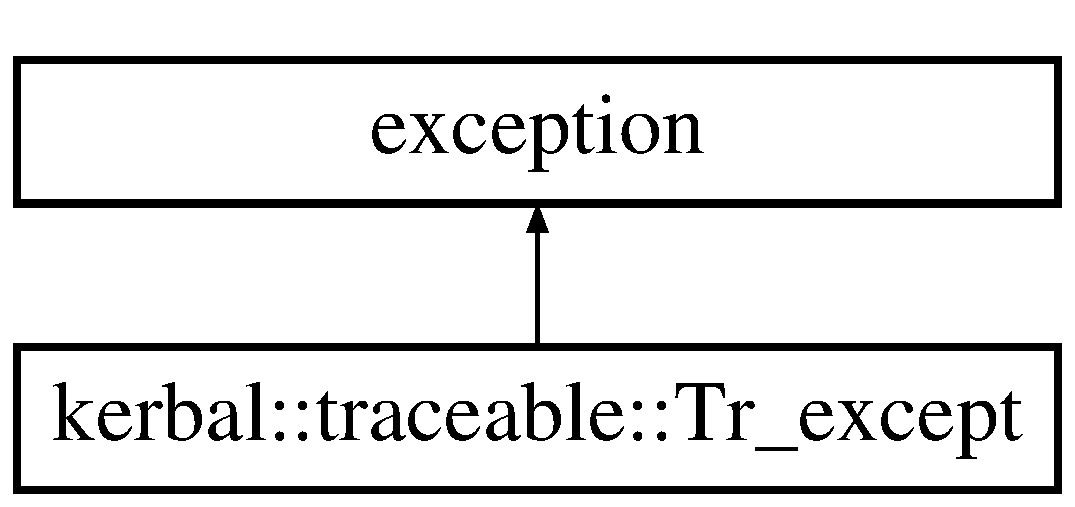
\includegraphics[height=2.000000cm]{classkerbal_1_1traceable_1_1_tr__except}
\end{center}
\end{figure}
\subsection*{类}
\begin{DoxyCompactItemize}
\item 
struct \hyperlink{structkerbal_1_1traceable_1_1_tr__except_1_1_trace}{Trace}
\end{DoxyCompactItemize}
\subsection*{Public 成员函数}
\begin{DoxyCompactItemize}
\item 
\mbox{\Hypertarget{classkerbal_1_1traceable_1_1_tr__except_a1f6b8bf28b4409c46120179d8650ba93}\label{classkerbal_1_1traceable_1_1_tr__except_a1f6b8bf28b4409c46120179d8650ba93}} 
{\bfseries Tr\+\_\+except} (const std\+::string \&\+\_\+\+M\+\_\+msg=\char`\"{}\char`\"{}, const std\+::string \&function\+\_\+name=\char`\"{}Unknown Function\char`\"{}, const std\+::string \&file\+\_\+name=\char`\"{}Unknown File\char`\"{}, int line=0)
\item 
\mbox{\Hypertarget{classkerbal_1_1traceable_1_1_tr__except_a7ff395a73c9b6721aa1847d2486239fc}\label{classkerbal_1_1traceable_1_1_tr__except_a7ff395a73c9b6721aa1847d2486239fc}} 
virtual const char $\ast$ {\bfseries what} () const \+\_\+\+G\+L\+I\+B\+C\+X\+X\+\_\+\+T\+X\+N\+\_\+\+S\+A\+F\+E\+\_\+\+D\+YN \+\_\+\+G\+L\+I\+B\+C\+X\+X\+\_\+\+U\+S\+E\+\_\+\+N\+O\+E\+X\+C\+E\+PT
\item 
\mbox{\Hypertarget{classkerbal_1_1traceable_1_1_tr__except_aa2fb4e5783dff16dbe387f9f42dcdfe0}\label{classkerbal_1_1traceable_1_1_tr__except_aa2fb4e5783dff16dbe387f9f42dcdfe0}} 
virtual void {\bfseries print\+\_\+trace} (std\+::ostream \&out=std\+::cerr) const
\item 
\mbox{\Hypertarget{classkerbal_1_1traceable_1_1_tr__except_af9315fa0298224e090578387935962be}\label{classkerbal_1_1traceable_1_1_tr__except_af9315fa0298224e090578387935962be}} 
virtual void {\bfseries re\+\_\+throw} (const std\+::string \&catch\+\_\+function\+\_\+name=\char`\"{}Unknown Function\char`\"{}, const std\+::string \&file\+\_\+name=\char`\"{}Unknown File\char`\"{}, int line=0) const
\end{DoxyCompactItemize}
\subsection*{Protected 属性}
\begin{DoxyCompactItemize}
\item 
\mbox{\Hypertarget{classkerbal_1_1traceable_1_1_tr__except_aef1f72279bbadc6f3cc6b8a9c36ec9ab}\label{classkerbal_1_1traceable_1_1_tr__except_aef1f72279bbadc6f3cc6b8a9c36ec9ab}} 
std\+::string {\bfseries \+\_\+\+M\+\_\+msg}
\item 
\mbox{\Hypertarget{classkerbal_1_1traceable_1_1_tr__except_a12f0843851f04e842237dd9852ce9fe6}\label{classkerbal_1_1traceable_1_1_tr__except_a12f0843851f04e842237dd9852ce9fe6}} 
std\+::list$<$ \hyperlink{structkerbal_1_1traceable_1_1_tr__except_1_1_trace}{Trace} $>$ {\bfseries trace\+\_\+record}
\end{DoxyCompactItemize}


该类的文档由以下文件生成\+:\begin{DoxyCompactItemize}
\item 
src/kerbal/Trexcept.\+hpp\item 
src/kerbal/Trexcept.\+cpp\end{DoxyCompactItemize}

\hypertarget{structkerbal_1_1traceable_1_1_tr__except_1_1_trace}{}\section{kerbal\+:\+:traceable\+:\+:Tr\+\_\+except\+:\+:Trace结构体 参考}
\label{structkerbal_1_1traceable_1_1_tr__except_1_1_trace}\index{kerbal\+::traceable\+::\+Tr\+\_\+except\+::\+Trace@{kerbal\+::traceable\+::\+Tr\+\_\+except\+::\+Trace}}
\subsection*{Public 成员函数}
\begin{DoxyCompactItemize}
\item 
\mbox{\Hypertarget{structkerbal_1_1traceable_1_1_tr__except_1_1_trace_aacad5214700c1ede35b8f040d396e415}\label{structkerbal_1_1traceable_1_1_tr__except_1_1_trace_aacad5214700c1ede35b8f040d396e415}} 
{\bfseries Trace} (std\+::string func\+\_\+name=\char`\"{}Unknown Function\char`\"{}, std\+::string file\+\_\+name=\char`\"{}Unknown File\char`\"{}, int line=0)
\end{DoxyCompactItemize}
\subsection*{Public 属性}
\begin{DoxyCompactItemize}
\item 
\mbox{\Hypertarget{structkerbal_1_1traceable_1_1_tr__except_1_1_trace_a4946f32b070a0bc288acfbe982154a0a}\label{structkerbal_1_1traceable_1_1_tr__except_1_1_trace_a4946f32b070a0bc288acfbe982154a0a}} 
std\+::string {\bfseries func\+\_\+name}
\item 
\mbox{\Hypertarget{structkerbal_1_1traceable_1_1_tr__except_1_1_trace_a8dbad22ac15fbae1c3d8bd8d03520572}\label{structkerbal_1_1traceable_1_1_tr__except_1_1_trace_a8dbad22ac15fbae1c3d8bd8d03520572}} 
std\+::string {\bfseries file\+\_\+name}
\item 
\mbox{\Hypertarget{structkerbal_1_1traceable_1_1_tr__except_1_1_trace_a11bd6453d09569ee05832e73b45507d0}\label{structkerbal_1_1traceable_1_1_tr__except_1_1_trace_a11bd6453d09569ee05832e73b45507d0}} 
int {\bfseries line}
\end{DoxyCompactItemize}


该结构体的文档由以下文件生成\+:\begin{DoxyCompactItemize}
\item 
src/kerbal/Trexcept.\+hpp\end{DoxyCompactItemize}

\chapter{文件说明}
\hypertarget{matrix_8hpp}{}\section{src/kerbal/math/matrix.hpp 文件参考}
\label{matrix_8hpp}\index{src/kerbal/math/matrix.\+hpp@{src/kerbal/math/matrix.\+hpp}}


本文件提供了对基本矩阵计算的支持  


{\ttfamily \#include $<$fstream$>$}\newline
{\ttfamily \#include $<$iostream$>$}\newline
{\ttfamily \#include $<$cmath$>$}\newline
{\ttfamily \#include \char`\"{}../array\+\_\+2d.\+hpp\char`\"{}}\newline
\subsection*{类}
\begin{DoxyCompactItemize}
\item 
class \hyperlink{classkerbal_1_1math_1_1_matrix}{kerbal\+::math\+::\+Matrix}
\begin{DoxyCompactList}\small\item\em 矩阵类 \end{DoxyCompactList}\end{DoxyCompactItemize}
\subsection*{命名空间}
\begin{DoxyCompactItemize}
\item 
 \hyperlink{namespacekerbal}{kerbal}
\begin{DoxyCompactList}\small\item\em kerbal 库 \end{DoxyCompactList}\item 
 \hyperlink{namespacekerbal_1_1math}{kerbal\+::math}
\begin{DoxyCompactList}\small\item\em 数学计算子库 \end{DoxyCompactList}\end{DoxyCompactItemize}
\subsection*{函数}
\begin{DoxyCompactItemize}
\item 
void {\bfseries std\+::swap} (\hyperlink{classkerbal_1_1math_1_1_matrix}{kerbal\+::math\+::\+Matrix} \&a, \hyperlink{classkerbal_1_1math_1_1_matrix}{kerbal\+::math\+::\+Matrix} \&b)
\begin{DoxyCompactList}\small\item\em 交换两个矩阵 \end{DoxyCompactList}\item 
\mbox{\Hypertarget{namespacekerbal_1_1math_aac8c0ee9511d7ac59fdca86e0d7a5ef9}\label{namespacekerbal_1_1math_aac8c0ee9511d7ac59fdca86e0d7a5ef9}} 
{\footnotesize template$<$size\+\_\+t N$>$ }\\const Matrix {\bfseries kerbal\+::math\+::cat} (const Matrix(\&a)\mbox{[}N\mbox{]})  throw (std\+::invalid\+\_\+argument)
\item 
\mbox{\Hypertarget{namespacekerbal_1_1math_ab0c3317760651c36ccae631e6826ff32}\label{namespacekerbal_1_1math_ab0c3317760651c36ccae631e6826ff32}} 
const Matrix {\bfseries kerbal\+::math\+::rotate\+\_\+X} (double sigma)
\item 
\mbox{\Hypertarget{namespacekerbal_1_1math_a8ae35ffad8d30503414300f7461e50d6}\label{namespacekerbal_1_1math_a8ae35ffad8d30503414300f7461e50d6}} 
const Matrix {\bfseries kerbal\+::math\+::rotate\+\_\+Y} (double sigma)
\item 
\mbox{\Hypertarget{namespacekerbal_1_1math_a4380bab6442decaf30f51695058e42da}\label{namespacekerbal_1_1math_a4380bab6442decaf30f51695058e42da}} 
const Matrix {\bfseries kerbal\+::math\+::rotate\+\_\+Z} (double sigma)
\item 
\mbox{\Hypertarget{namespacekerbal_1_1math_a37e3d41de6613f1820954b46fc431762}\label{namespacekerbal_1_1math_a37e3d41de6613f1820954b46fc431762}} 
void {\bfseries kerbal\+::math\+::rotate\+\_\+X} (double sigma, const double \&x0, double \&y0, double \&z0)  throw ()
\item 
\mbox{\Hypertarget{namespacekerbal_1_1math_a128fd0aa8828144d753d6d000dba8406}\label{namespacekerbal_1_1math_a128fd0aa8828144d753d6d000dba8406}} 
void {\bfseries kerbal\+::math\+::rotate\+\_\+Y} (double sigma, double \&x0, const double \&y0, double \&z0)  throw ()
\item 
\mbox{\Hypertarget{namespacekerbal_1_1math_ae2c2044405fa1e952ccb07dae1a61111}\label{namespacekerbal_1_1math_ae2c2044405fa1e952ccb07dae1a61111}} 
void {\bfseries kerbal\+::math\+::rotate\+\_\+Z} (double sigma, double \&x0, double \&y0, const double \&z0)  throw ()
\end{DoxyCompactItemize}


\subsection{详细描述}
本文件提供了对基本矩阵计算的支持 

\begin{DoxyAuthor}{作者}
倪文卿 
\end{DoxyAuthor}
\begin{DoxyDate}{日期}
2017-\/4-\/30 
\end{DoxyDate}
\begin{DoxyCopyright}{版权所有}
倪文卿 

\href{http://thinkspirit.org/}{\tt Think\+Spirit Laboratory} of \href{http://www.nuist.edu.cn/}{\tt Nanjing University of Information Science \& Technology}  
\end{DoxyCopyright}


\subsection{函数说明}
\mbox{\Hypertarget{matrix_8cpp_file_abf53e915d879b9a0ba35b7d3e6fd6f8b}\label{matrix_8cpp_file_abf53e915d879b9a0ba35b7d3e6fd6f8b}} 
\index{matrix.\+hpp@{matrix.\+hpp}!swap@{swap}}
\index{swap@{swap}!matrix.\+hpp@{matrix.\+hpp}}
\subsubsection{\texorpdfstring{swap()}{swap()}}
{\footnotesize\ttfamily void std\+::swap (\begin{DoxyParamCaption}\item[{\hyperlink{classkerbal_1_1math_1_1_matrix}{kerbal\+::math\+::\+Matrix} \&}]{a,  }\item[{\hyperlink{classkerbal_1_1math_1_1_matrix}{kerbal\+::math\+::\+Matrix} \&}]{b }\end{DoxyParamCaption})}



交换两个矩阵 


\begin{DoxyParams}{参数}
{\em a} & 矩阵 a \\
\hline
{\em b} & 矩阵 b \\
\hline
\end{DoxyParams}
\begin{DoxyRemark}{备注}
重载了标准命名空间中的 swap 函数, 使得两个矩阵的交换操作能在 O(1) 的时间复杂度中完成 
\end{DoxyRemark}

%--- End generated contents ---

% Index
\backmatter
\newpage
\phantomsection
\clearemptydoublepage
\addcontentsline{toc}{chapter}{索引}
\printindex

\end{document}
